\chapter{Fatigue Damage due to Waves}
\label{chap:enviroment}
This section will give a very brief insight in the concepts that are relevant in this project thesis. The theory in this section is taken from \cite{Faltinsen1990}.  For linear theory, the results from irregular waves can be obtained by adding together results from regular waves. For long-crested irregular sea, the wave elevation ca be described as:
\begin{equation}
    \zeta = \sum_{j-1}^N A_j \sin(\omega_jt-k_jx+\epsilon_j)
    \label{eq:elevation}
\end{equation}
\cite{Faltinsen1990}
Where $\omega$ is the circular frequency, $t$ is time, $k$ is the wave number, $\epsilon$ is the wave number and $A$ is the the amplitude that can also be expressed in terms of the wave spectrum:
\begin{equation}
    \frac{1}{2}A_j=S(\omega_j) \Delta \omega
\end{equation}
Where $\Delta \omega$ is the difference between successive frequencies. The wave elevation is Gaussian distributed with mean at zero and $\sigma^2= \int_0 ^ \infty S(\omega) d\omega $. The wave spectrum assumes that the sea can be describes as a stationary random process, meaning that it is a short-time description of the sea state. The sea state is defined by the sigificant wave height, Hs and the peak period, Tp. Hs is the mean height of the $\frac{1}{3}$ highest waves in the sea state, and Tp is the peak frequency of the wave spectrum. There excists several different spectums but according to \cite{Lifes50+D1.1} the JONSWAP (Joint North Sea Wave Project) is suitable for "wind seas", and thus this is what will be used in this case. The JONSWAP apectrum can be described as:
\begin{equation}
    S(\omega)=155 \frac{H_s^2}{T_1^4 \omega ^5} \exp{(\frac{-994}{T_1^4 \omega ^4})} 3.3^Y
\end{equation}
Where
\begin{equation}
    Y= \exp \left(-\left( \frac{0.191 \omega T_1 -1}{2^\frac{1}{2} \sigma} \right)^2\right)
\end{equation}

\begin{figure}[H]
\subfloat[General Wave Spectrum \label{fig:lm_total}]
  {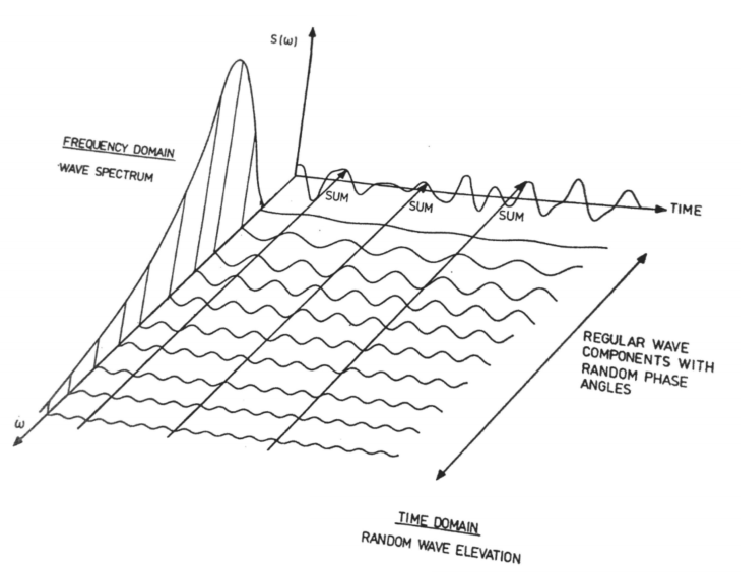
\includegraphics[width=.45\linewidth]{figures/spectrum}}\hfill
\subfloat[JONSWAP Wave Spectrum \label{fig:lm_cross}]
  {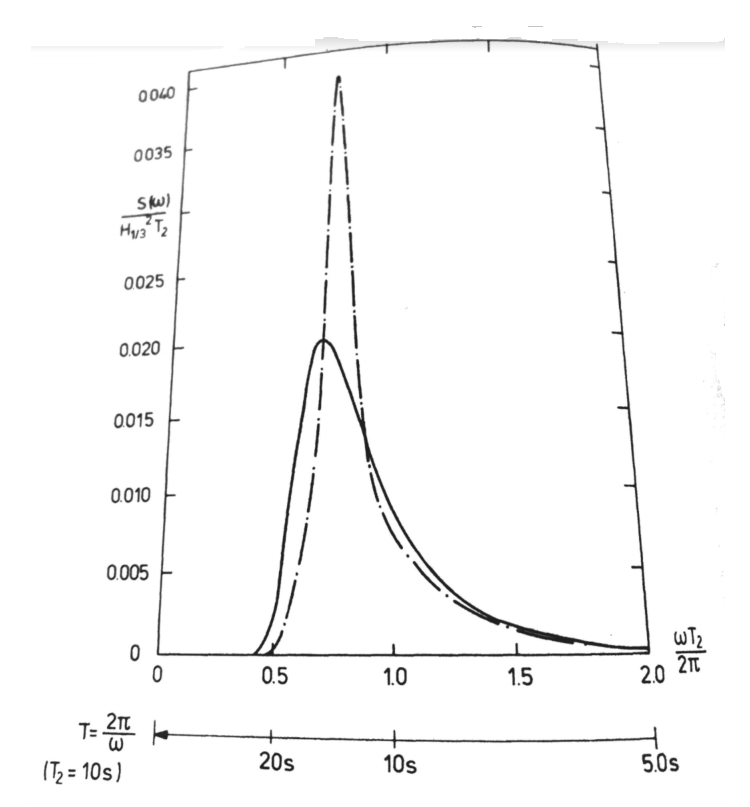
\includegraphics[width=.35\linewidth]{figures/JONSWAP}}\hfill
\caption{General wave spectrum and JONSWAP Spectrum \cite{Faltinsen1990}}
\label{fig:spectrum}
\end{figure}

The long term sea state is often described in a scatter diagram featuring the number of occurrences for different Hs and the Tp.  \newline
\newline